\chapter{Race LogicとCMOSによる実装}
本章では,まずRace Logicの基本原理を説明する.
具体的な評価の対象アプリケーションである配列アラインメントと
CMOSによる実装例をまとめ,
その後Race Logicの検討において解決すべき課題について述べる.

\section{Race Logic}
Race Logicの基本概念は,回路に設定された競争条件を利用して,計算を実行することである.
Race Logicの計算は有向非巡回グラフ
(Directed Acyclic Graph)の最短・最長経路探索に帰結する.
有向非巡回グラフとは,グラフ理論における閉路のない有向グラフの事である.
その例を図\ref{fig:DAG}に示す.
\begin{figure}[t!]
\begin{center}
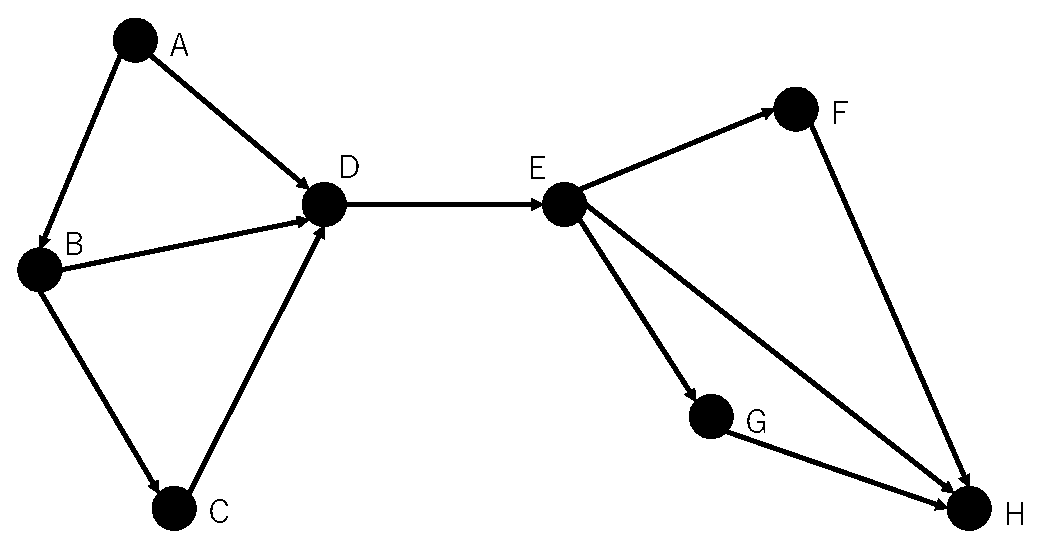
\includegraphics[keepaspectratio,scale=0.5]{fig/2/DAG.eps}
\caption{有向非巡回グラフの例}
\label{fig:DAG}
\end{center}
\end{figure}
有向グラフは頂点と有向辺から構成される.
その中でも,辺は点同士をつなぐが,ある頂点 v から出発し辺をたどっても頂点 v に戻ってこないというものが
有向非巡回グラフである.
ある頂点から別の頂点までの経路をパスと呼ぶ.
Race logicでは最短・最長経路を探索するために,始点から終点までの各パスにおいて条件に合わせて重み付けを行い,出力時にその重みの総和を見る.
その総和の最小値を見るか最大値を見るかが,最短・最長経路探索にそれぞれ対応している.

重みに遅延時間を選択することによって,各パスを通過する信号毎に入力から出力までの伝搬時間が変わってくる.
信号がRace Logicを用いた回路に入力されてから出力されるまでの回路伝搬遅延時間を計測することが,パスの重みの総和を見ることに等しい.
最短経路検索においては一番早く出力された信号の回路伝搬遅延時間を,
最長経路検索においては一番遅く出力された信号の回路伝搬遅延時間のみを見る.
つまり,出力のタイミングを競うレースに勝利した信号の回路伝搬遅延時間のみを見る,ということであり,Race Logicの名前の所以でもある.
出力信号の遅延時間がとある情報を持つ計算結果となる.
例として,図\ref{fig:DAG1}の頂点Aに信号を入力し,
頂点Hから出力されるものを考える.
\begin{figure}[t!]
\begin{center}
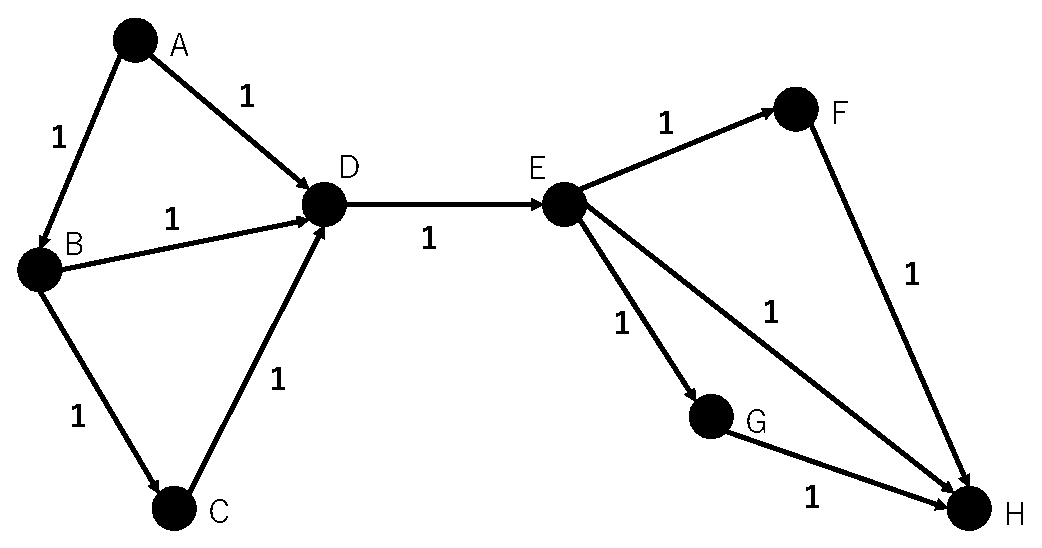
\includegraphics[keepaspectratio,scale=0.5]{fig/2/DAG1.eps}
\caption{Race Logicの例}
\label{fig:DAG1}
\end{center}
\end{figure}
これは図\ref{fig:DAG}の一辺を通過する際の遅延時間を1としたものである.
頂点Aに信号を入力してから頂点Hに至る経路は,
A→D→E→F→G,A→D→E→G→H,A→D→E→H,
A→B→D→E→F→G,A→B→D→E→G→H,A→B→D→E→H,
A→B→C→D→E→F→G,A→B→C→D→E→G→H,A→B→C→D→E→Hの9通り考えられ,
各経路を通った信号の遅延時間はそれぞれ4,4,3,5,5,4,6,6,5である.
よって最短経路はA→D→E→Hであり,一番最初に出力される信号の遅延時間は3である.
一辺の通過の際の遅延時間を1としたので,
一番最初に出力された信号の遅延時間は頂点Aから頂点Hまでの距離を表している.

このように出力信号の遅延時間はとある情報を持っており,
どのような情報を持つかは応用するアプリケーションによって異なる.

\section{配列アラインメント}
生物学の分野において注目されている生物配列(DNAの塩基配列とタンパク質アミノ酸配列) の文字列処理(配列情報解析)
\cite{浅井潔2000配列情報と確立モデル,後藤修1998マルチプルアラインメントは生体高分子情報の交差点}
の中でも,配列アラインメントに焦点を当てる.

DNAやタンパク質はユニットと名付けられた単位の物質が一列に並んだ高分子である.
ここでいうユニットとは,DNAにおいては4種の核酸,タンパク質においては20種類のアミノ酸である.
それぞれのユニットを文字としDNAやタンパク質の配列を単なる文字列だとみなして
処理をしてもある種の本質は失われないという考えに基づき,
文字列処理をすることで生物配列の解析を行う.
DNAの塩基配列やタンパク質アミノ酸配列の研究は,
バイオインフォマティクスの最重要課題の一つとして取り組まれてきた.
配列情報解析の重要な対象であるゲノム塩基配列は,
すでに200種類以上が決定されており,さらに多くの解析が進行中であるといわれている
\cite{浅井潔2005バイオインフォマティクス}.

生物配列の文字列処理の中で,DNA配列中に同じ順序で並んでいるユニットのパターンを見つける
配列アラインメントがある\cite{須戸里織2011バイオインフォマティクスゲノム配列から
機能解析へバイオインフォマティクスゲノム配列から機能解析へ}.
アラインメントとは,複数の配列を入力として配列要素の間に最適な対応関係を求める処理である.
配列アラインメントの中には,グローバル配列アラインメントとローカル配列アラインメントがある.
グローバル配列アラインメントは,ある2つ以上の配列全体の間でのアラインメントを見つけることであり,
ローカル配列アラインメントは,ある2つ以上の配列の一部分で最も一致度が高い部分でのアラインメントを見つけることである.
例として,とある配列Pと配列Qのグローバル配列アラインメントとローカル配列アラインメントを図\ref{fig:grlc}に示す.
\begin{figure}[t!]
\begin{center}
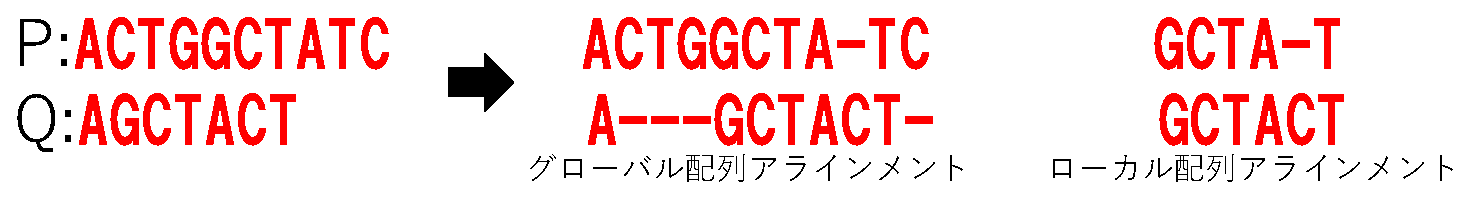
\includegraphics[keepaspectratio,scale=0.5]{fig/2/grlc.eps}
\caption{グローバル配列アラインメントとローカル配列アラインメント}
\label{fig:grlc}
\end{center}
\end{figure}

配列アラインメントには,動的計画法による解法としてNeedleman-Wunschアルゴリズム\cite{needleman1970general}やSmith-Watermanアルゴリズム\cite{smith1981identification}が存在する.
配列アラインメントは生物学において重要な手法であり,
計算機を用いた処理の高速化は従来より多くの研究がなされてきた\cite{須戸里織2011gpu,宗川裕馬2008統合開発環境,sandes2011smith,liu2015accelerating,伊野文彦2007gpu}.

文字列の類似度を知るための典型的な手法は,情報理論に由来する編集距離 (edit distance) である.
編集距離は,一方の文字列をもう一方の文字列に変形するのに必要な手順である一文字の挿入・削除・置換に
それぞれ編集スコアを割り当て,そのスコアの和として定義される.
編集距離の理解を助けるために,長さN = 5の文字列X= "TCGAT"と長さM = 5の文字列Y= "GTCAC"を考える.
\begin{figure}[t!]
\begin{center}
\subfigure[]{
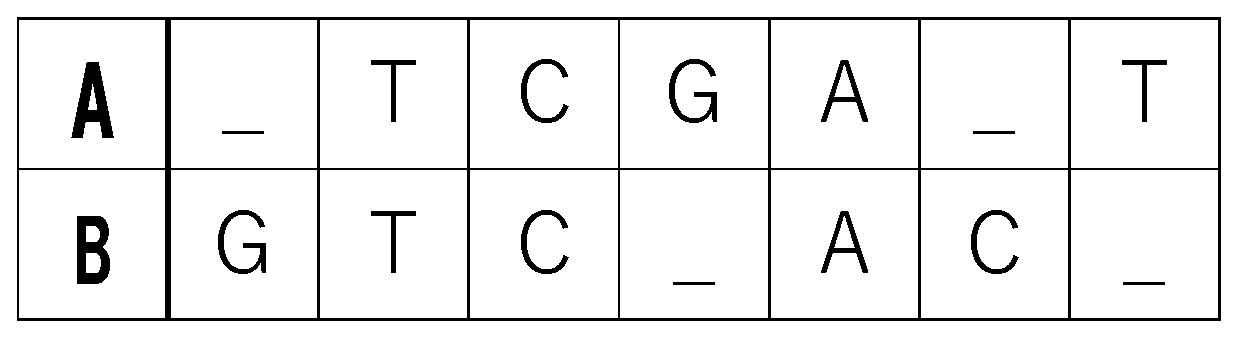
\includegraphics[keepaspectratio, scale=0.25]{fig/2/ed1.eps}
\label{fig:ed1}
 }
\subfigure[]{
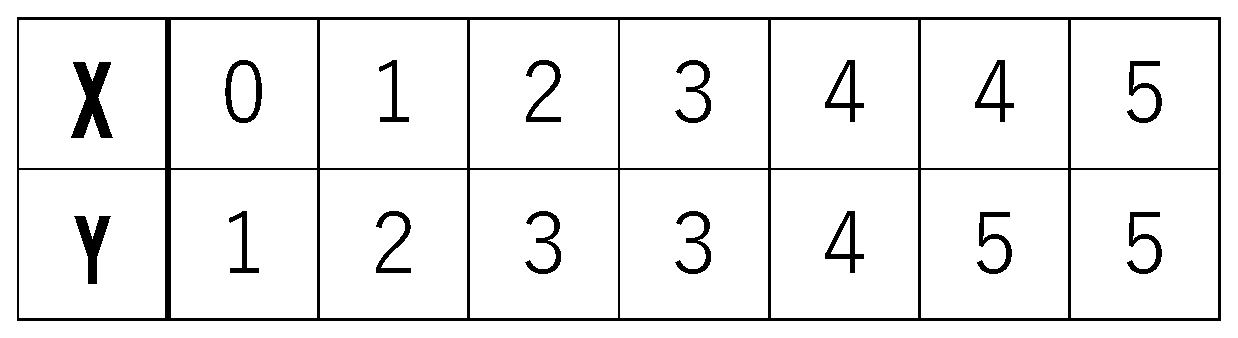
\includegraphics[keepaspectratio, scale=0.25]{fig/2/ed2.eps}
\label{fig:ed2}
 }\\
\subfigure[]{
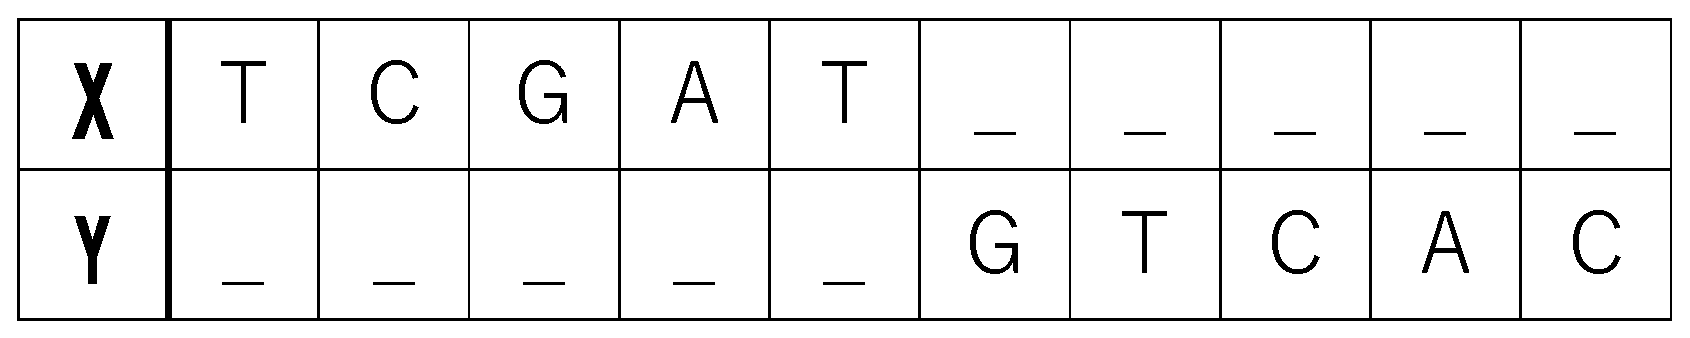
\includegraphics[keepaspectratio, scale=0.25]{fig/2/ed3.eps}
\label{fig:ed3}
 }
\subfigure[]{
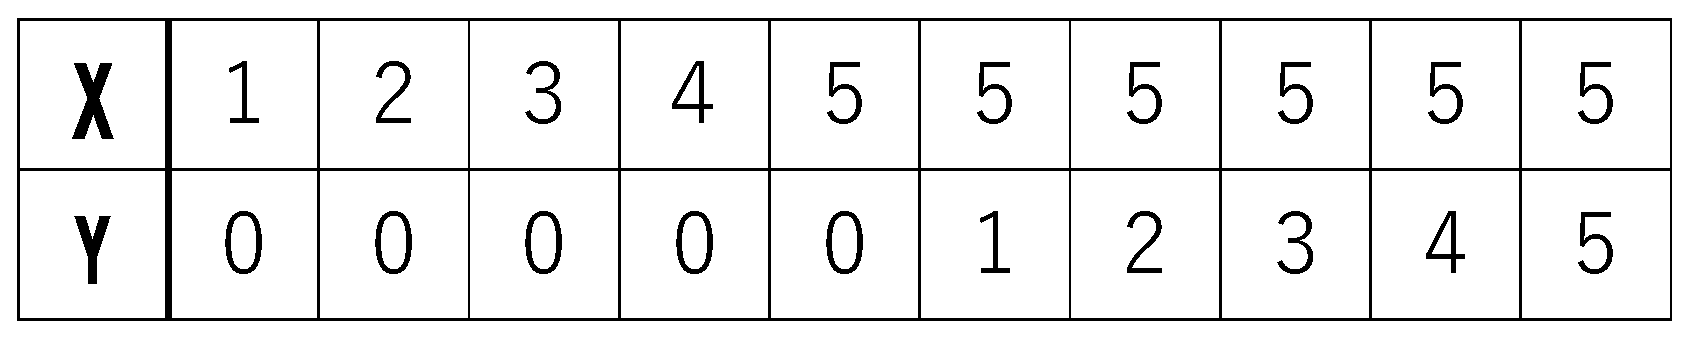
\includegraphics[keepaspectratio, scale=0.25]{fig/2/ed4.eps}
\label{fig:ed4}
 }\\
\subfigure[]{
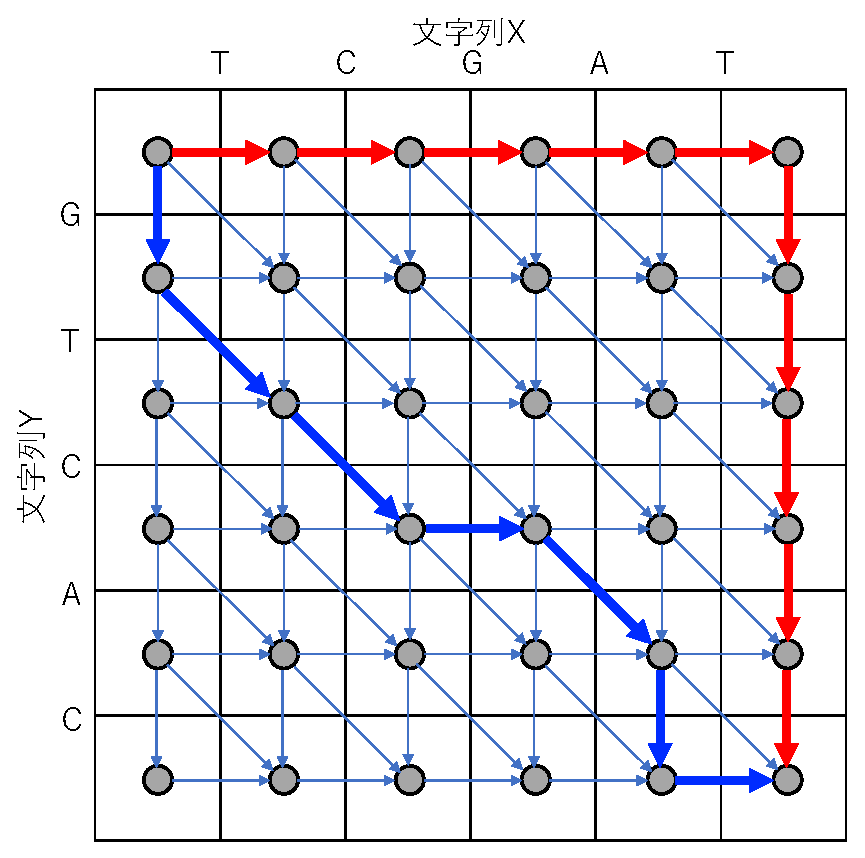
\includegraphics[keepaspectratio, scale=0.5]{fig/2/ed5.eps}
\label{fig:ed5}
 }
\caption{編集距離と編集グラフ}
\label{fig:ed}
\end{center}
\end{figure}
図\ref{fig:ed1}と図\ref{fig:ed3}は,文字列AをBに変換する2つの方法を示している.
上の行のスペースは挿入を表し,下の行のスペースは削除を表す.
両方の行に同じ文字がある列は一致と呼ぶ.
図\ref{fig:ed1}の方法は文字GとTを削除し,GとCを挿入する一方で,
図\ref{fig:ed3}の方法は文字列Aを完全に削除して文字列Bを挿入している.

図\ref{fig:ed2}および図\ref{fig:ed4}は, 2つのアラインメント方法の代替表現である.
任意の位置の数字は,図\ref{fig:ed1}および図\ref{fig:ed3}の方法においてその位置までに存
在する記号の数を示している.
この表示は各列の数値が図\ref{fig:ed5}に示す2次元の編集グラフの座標と考えることができる.
このグラフを編集グラフという.
編集グラフは2つの文字列間において,取りうる限りの配置の
二次元表現である有向非巡回グラフ(DAG)である.
全てのエッジが編集操作に対応していて,垂直の矢印は挿入を,水平の矢印は削除を,斜めの矢印は一致を表している.
任意のアラインメントはこのグラフのパスで表現できる.
例えば、図\ref{fig:ed5}の青と赤の矢印は,それぞれ図\ref{fig:ed1}および図\ref{fig:ed3}に示す2つのアライメントに対応している.

2つの文字列間の編集距離は,動的計画法を用いて計算できる.
動的計画法は小さな部分問題から始めて次第に大きな問題を漸進的に解決し,
各ステップはそれ以前の計算の結果に依存している.
編集グラフ上の各ノードは,部分問題の最適解に対応するスコア,
すなわち最初のノードから自身への最短経路に対応するスコアを計算している.
隣接するノードは,計算が対角線に沿って進むにつれてそれ以前の最適解を利用して
自身のスコアを計算する.
編集グラフ自体は最初のノードから最後のノードまでの経路として,
表現される可能性のあるすべてのアライメントから構成されている.
よって,上記の方法は比較対象の文字列間の最適なアライメントについて
空間全体の検索が保証されている.

任意の2つの文字列が与えられた場合,多数の異なるパスがあり,それぞれが独自のアラインメントを持つ.
ある特定のアライメントの相対的なメリットを決定するために
スコアマトリックスが導入される.
このスコアマトリックスは効果的に編集グラフの各エッジの重みを定義することができる.
スコアマトリックスとはあるユニット間の一致不一致や置換確率から求められる
スコアからなる行列である.
一致・不一致スコアと対数オッズスコアの式を式\ref{eq:mchun}と式\ref{eq:odds}にそれぞれ示す.
\begin{equation}
S(A,B)= \left \{
\begin{array}{l}
\alpha \ \ A = B\\
\beta \ \ A \neq B
\end{array}
\right.
\label{eq:mchun}
\end{equation}
\begin{equation}
S(A,B)= \log \cfrac{q(A,B)}{p(A)p(B)}
\label{eq:odds}
\end{equation}
$ここでq(A,B)は進化上の関係からAとBの対応が生じた確率,
p(A)は偶然にAが生じた確率,p(A)P(B)は偶然にAとBの対応が生じた確率である.$
図\ref{fig:scorematrix}には式\ref{eq:mchun}に具体的な数値を当てはめた場合のスコアマトリックス例を示す.
一般的に,不一致のペナルティは特定の文字のペアにも依存することに注意が必要で
ある.
\begin{figure}[t!]
\begin{center}
\subfigure[最長経路探索に用いられるスコアマトリックス]{
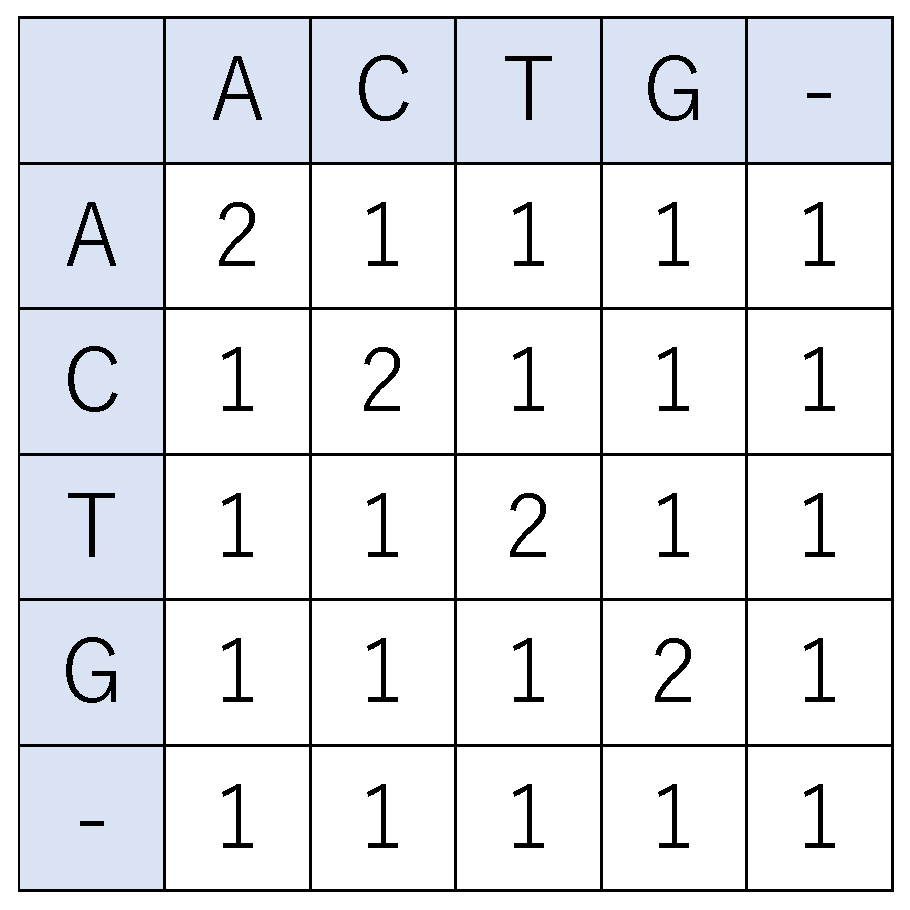
\includegraphics[keepaspectratio,scale=0.5]{fig/2/maxscore_ex.eps}
\label{fig:scorematrixmax}}
\subfigure[最短経路探索に用いられるスコアマトリックス]{
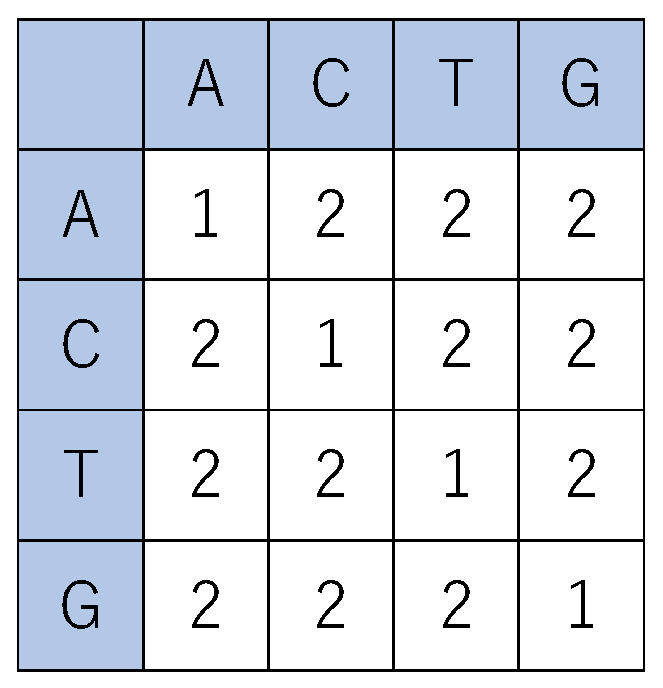
\includegraphics[keepaspectratio,scale=0.5]{fig/2/minscore_ex.eps}
\label{fig:scorematrixmin}}
\caption{スコアマトリックスの例}
\label{fig:scorematrix}
\end{center}
\end{figure}

あるノードにおけるスコアの最大値と最小値を求める関数は
式\ref{eq:maxscore}と式\ref{eq:minscore}のように書ける.
\begin{subequations}
\begin{align}
S_{i,j}= max \left \{
\begin{array}{l}
S_{i-1,j}+\delta(-,P_{j}) \\
S_{i,j-1}+\delta(Q_{i},-) \\
S_{i-1,j-1}+\delta(Q_{i},P_{j})
\end{array}
\right.\label{eq:maxscore} \\
S_{i,j}= min \left \{
\begin{array}{l}
S_{i-1,j}+\delta(-,P_{j}) \\
S_{i,j-1}+\delta(Q_{i},-) \\
S_{i-1,j-1}+\delta(Q_{i},P_{j})
\end{array}
\right.\label{eq:minscore}
\end{align}
\label{eq:minmaxscore}
\end{subequations}
iとjは図\ref{fig:ed5}に示す行と列のインデックスである.

アラインメントのメリットを決定することとはつまり,
図\ref{fig:scorematrixmax}のマトリックスと式\ref{eq:maxscore}を用いて最長経路を探索すること,
または図\ref{fig:scorematrixmin}のマトリックスと式\ref{eq:minscore}を用いて最短経路を探索することと等しい.

\section{CMOSによるRace Logic実装}
本節では,CMOSを用いたRace Logic実装例として,配列アラインメントアクセラレータを説明する.
Race Logicの考えを用いて実装された配列アラインメントアーキテクチャの基本構造を図\ref{fig:racelogicarray}に示す.
このRace Logic Arrayはセルと呼ばれる単位のユニットが繰り返される構造をとっている.
\begin{figure}[t!]
\begin{center}
\subfigure[Race Logicを用いた配列アラインメントアクセラレータの構成]{
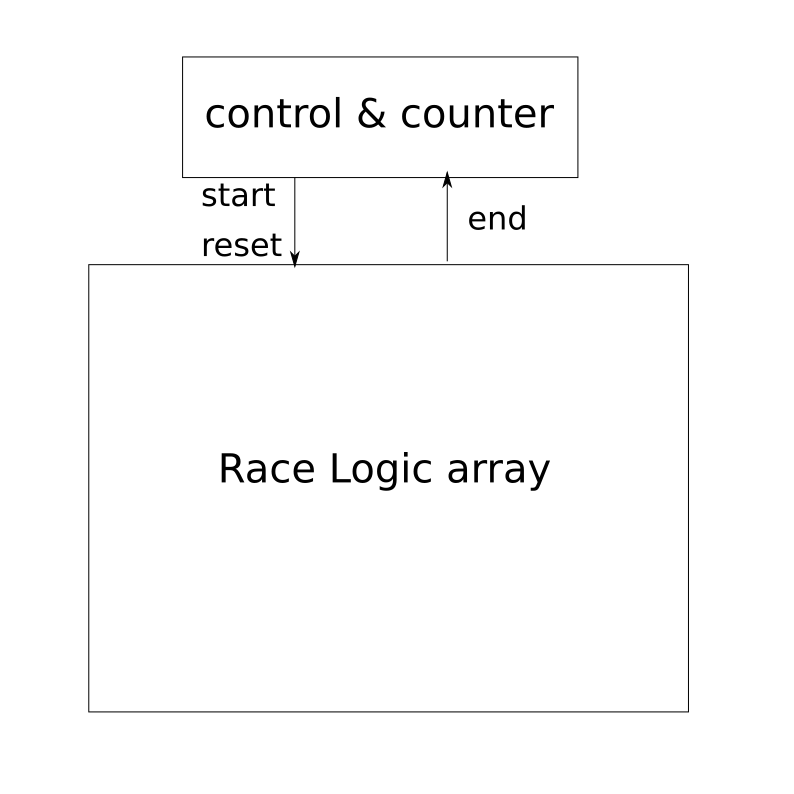
\includegraphics[keepaspectratio,scale=0.3]{fig/2/lightracelogic_1.png}
\label{fig:ctrl}}
\subfigure[Race Logic Arrayの構成]{
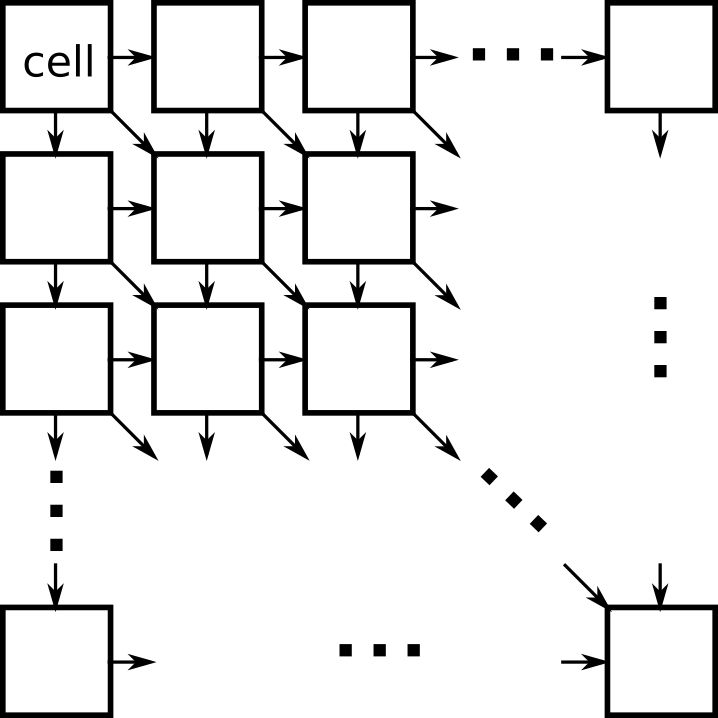
\includegraphics[keepaspectratio,scale=0.3]{fig/2/lightracelogic_2.png}}
\caption{配列アラインメントアクセラレータの基本構造}
\label{fig:racelogicarray}
\end{center}
\end{figure}
図\ref{fig:ed5}に示す編集グラフに対して,Race Logic Arrayが編集グラフ全体に,セルがノードに対応する.
セルは上・斜上・左のセルから信号の入力を受け付ける.
信号が入力された後,設定された条件に合わせて適切な処理をした後に,
次のセルへと信号を出力する.
実装の選択肢として,セルへの信号伝搬をクロックと同期させる同期型と,セルへの信号伝搬をクロックと同期させない非同期型とがある.

最短経路探索を行うことでDNAグローバル配列アラインメントスコアを得る配列アラインメントアクセラレータについて,同期型と非同期型を見ていく.

\begin{itemize}
\item CMOSによる同期型Race Logic実装\\
CMOSで実装された同期型Race Logicのセルの構造を図\ref{fig:CMOSsync}に示す.
\begin{figure}[t!]
\begin{center}
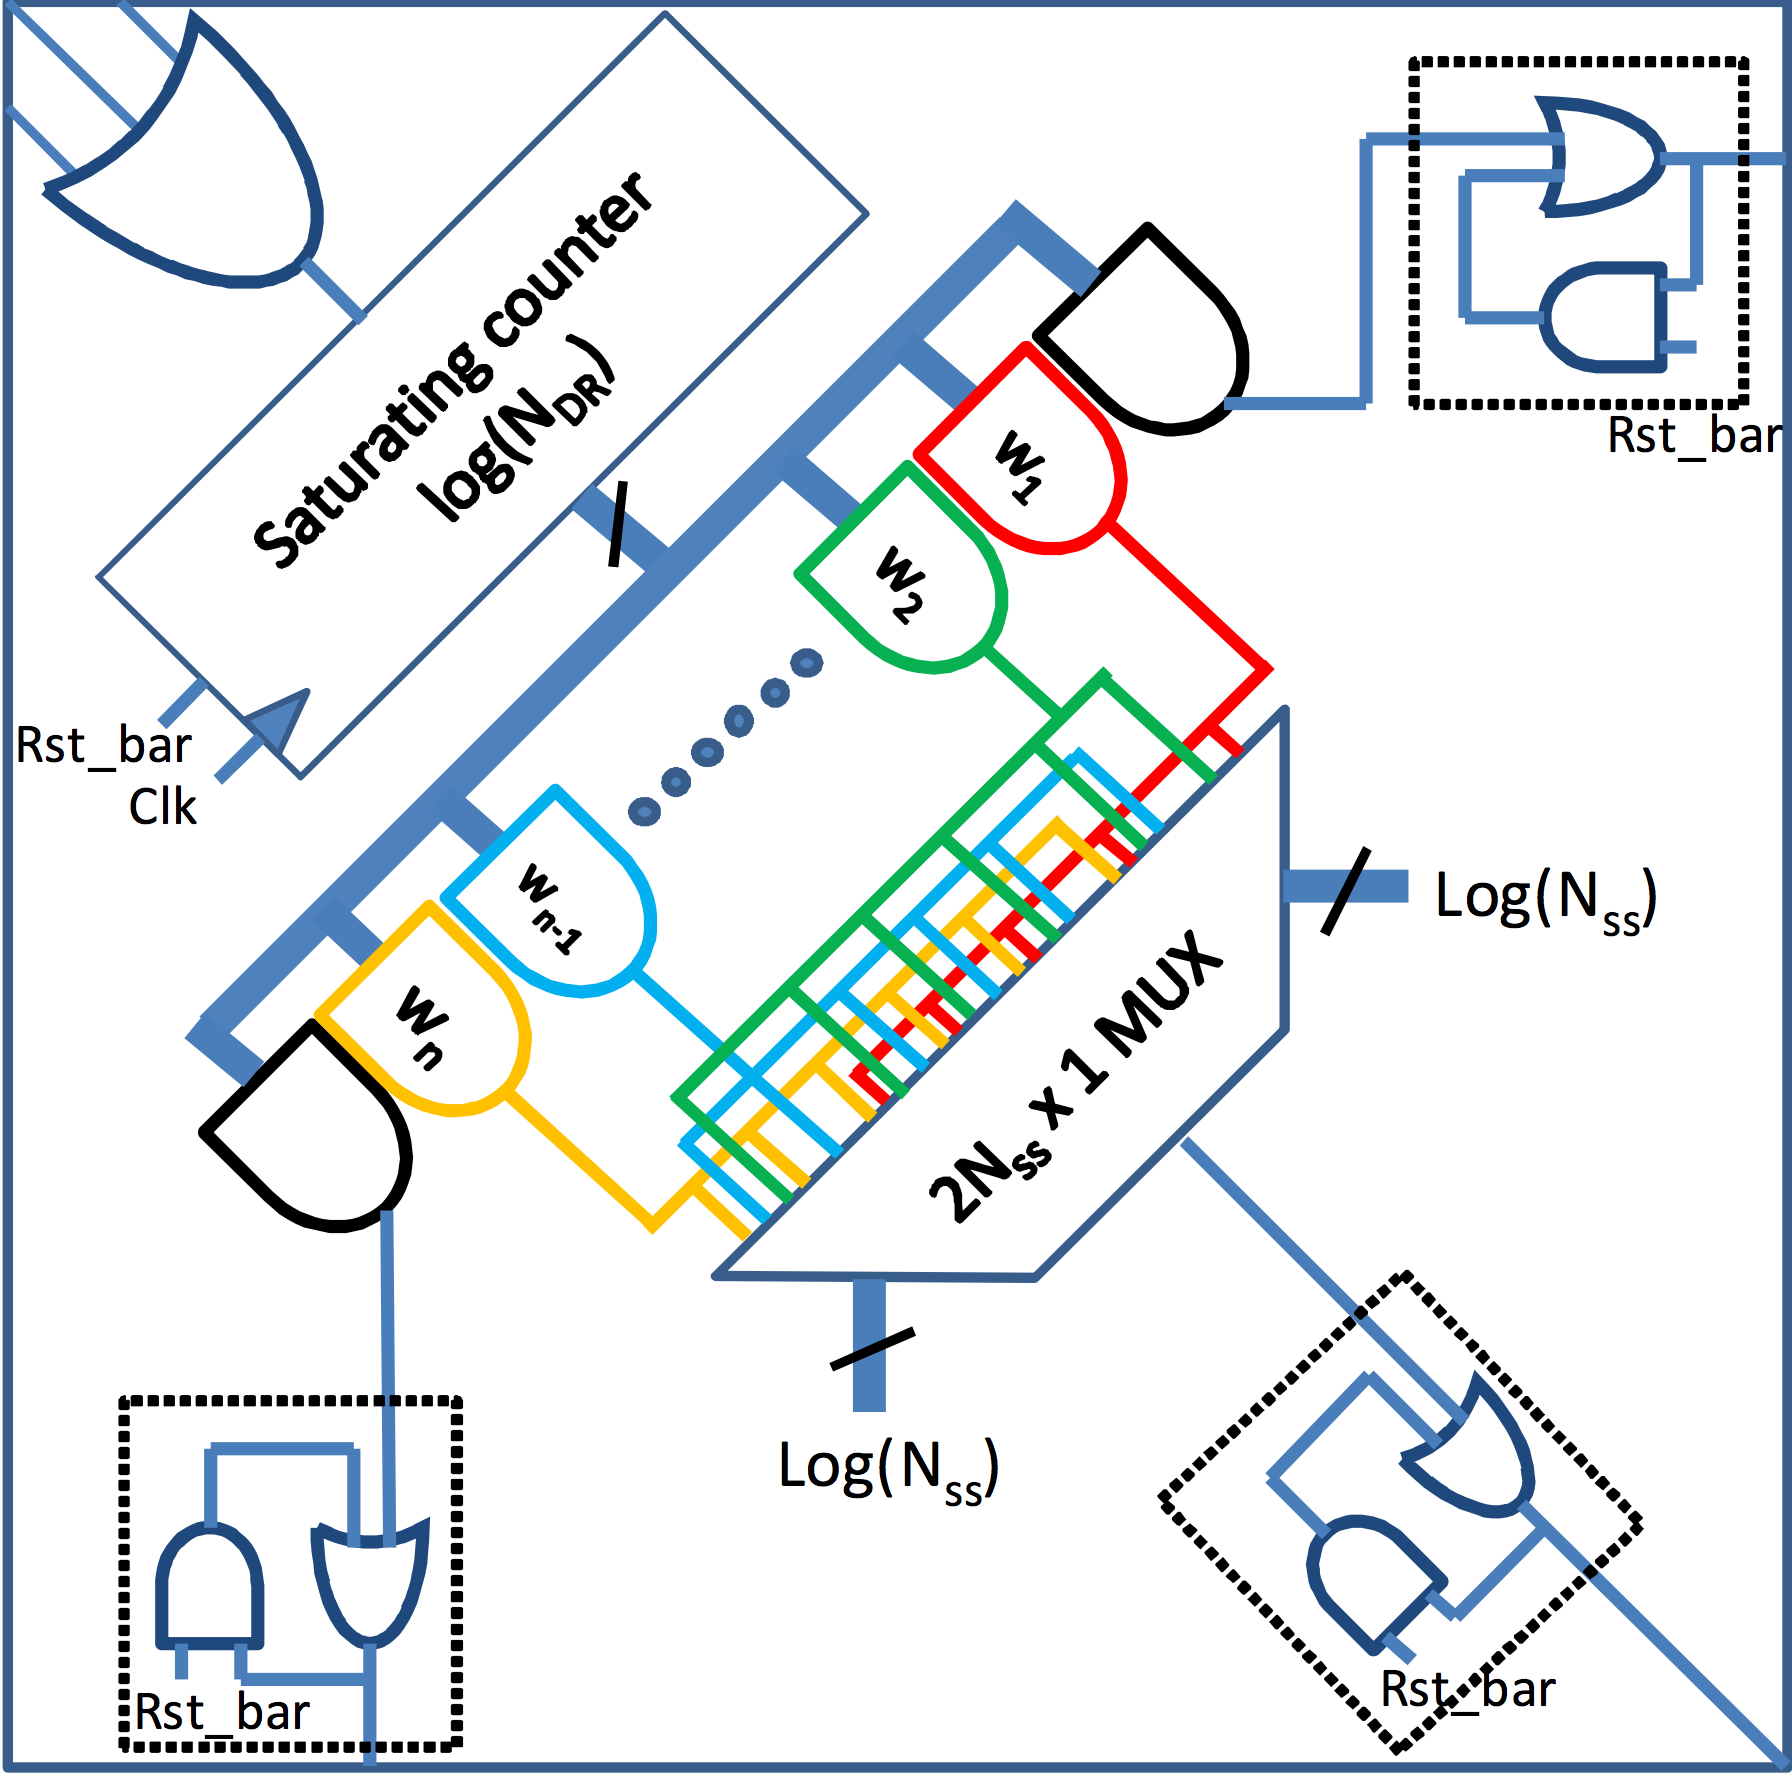
\includegraphics[keepaspectratio,scale=0.3]{fig/2/CMOSsync.png}
\caption{CMOSで実装された同期型Race Logicのセル構造\cite{madhavan2014race}}
\label{fig:CMOSsync}
\end{center}
\end{figure}

ブール値“1”の信号は左・斜上・上のセルのいずれからも入力される.
入力された信号はORゲートを通過して、飽和アップカウンタにおいてNクロックサイクルに0をカウントする.この飽和アップカウンタをクロックと同期させる.
これにより,1つのセルを通過し,右・下のセルへと伝搬する際に1クロックサイクルを要する.
各着色ゲートでは伝搬信号に対してそれぞれ違う伝搬遅延時間を付加し,
MUXで所望の伝搬遅延時間を付加するゲートからの出力を選択することができる.
生成される出力信号がパルスではなく固定ブール値“1”であることを確実にするために,到着回路のセットが配置され,各計算の最後にリセットされている.

図\ref{fig:CMOSsync}のセルを繰り返した構造を持つアレイに信号が入力された時から出力信号を得るまでのクロック数をカウントするカウンタがアレイ外部に存在する.
このカウンタが計測した値が最短経路をパスした時のクロック数となる.

\item CMOSによる非同期型Race Logic実装\\
CMOSで実装された非同期型Race Logicのセルの構造を図\ref{fig:CMOSasync}に示す.
\begin{figure}[t!]
\begin{center}
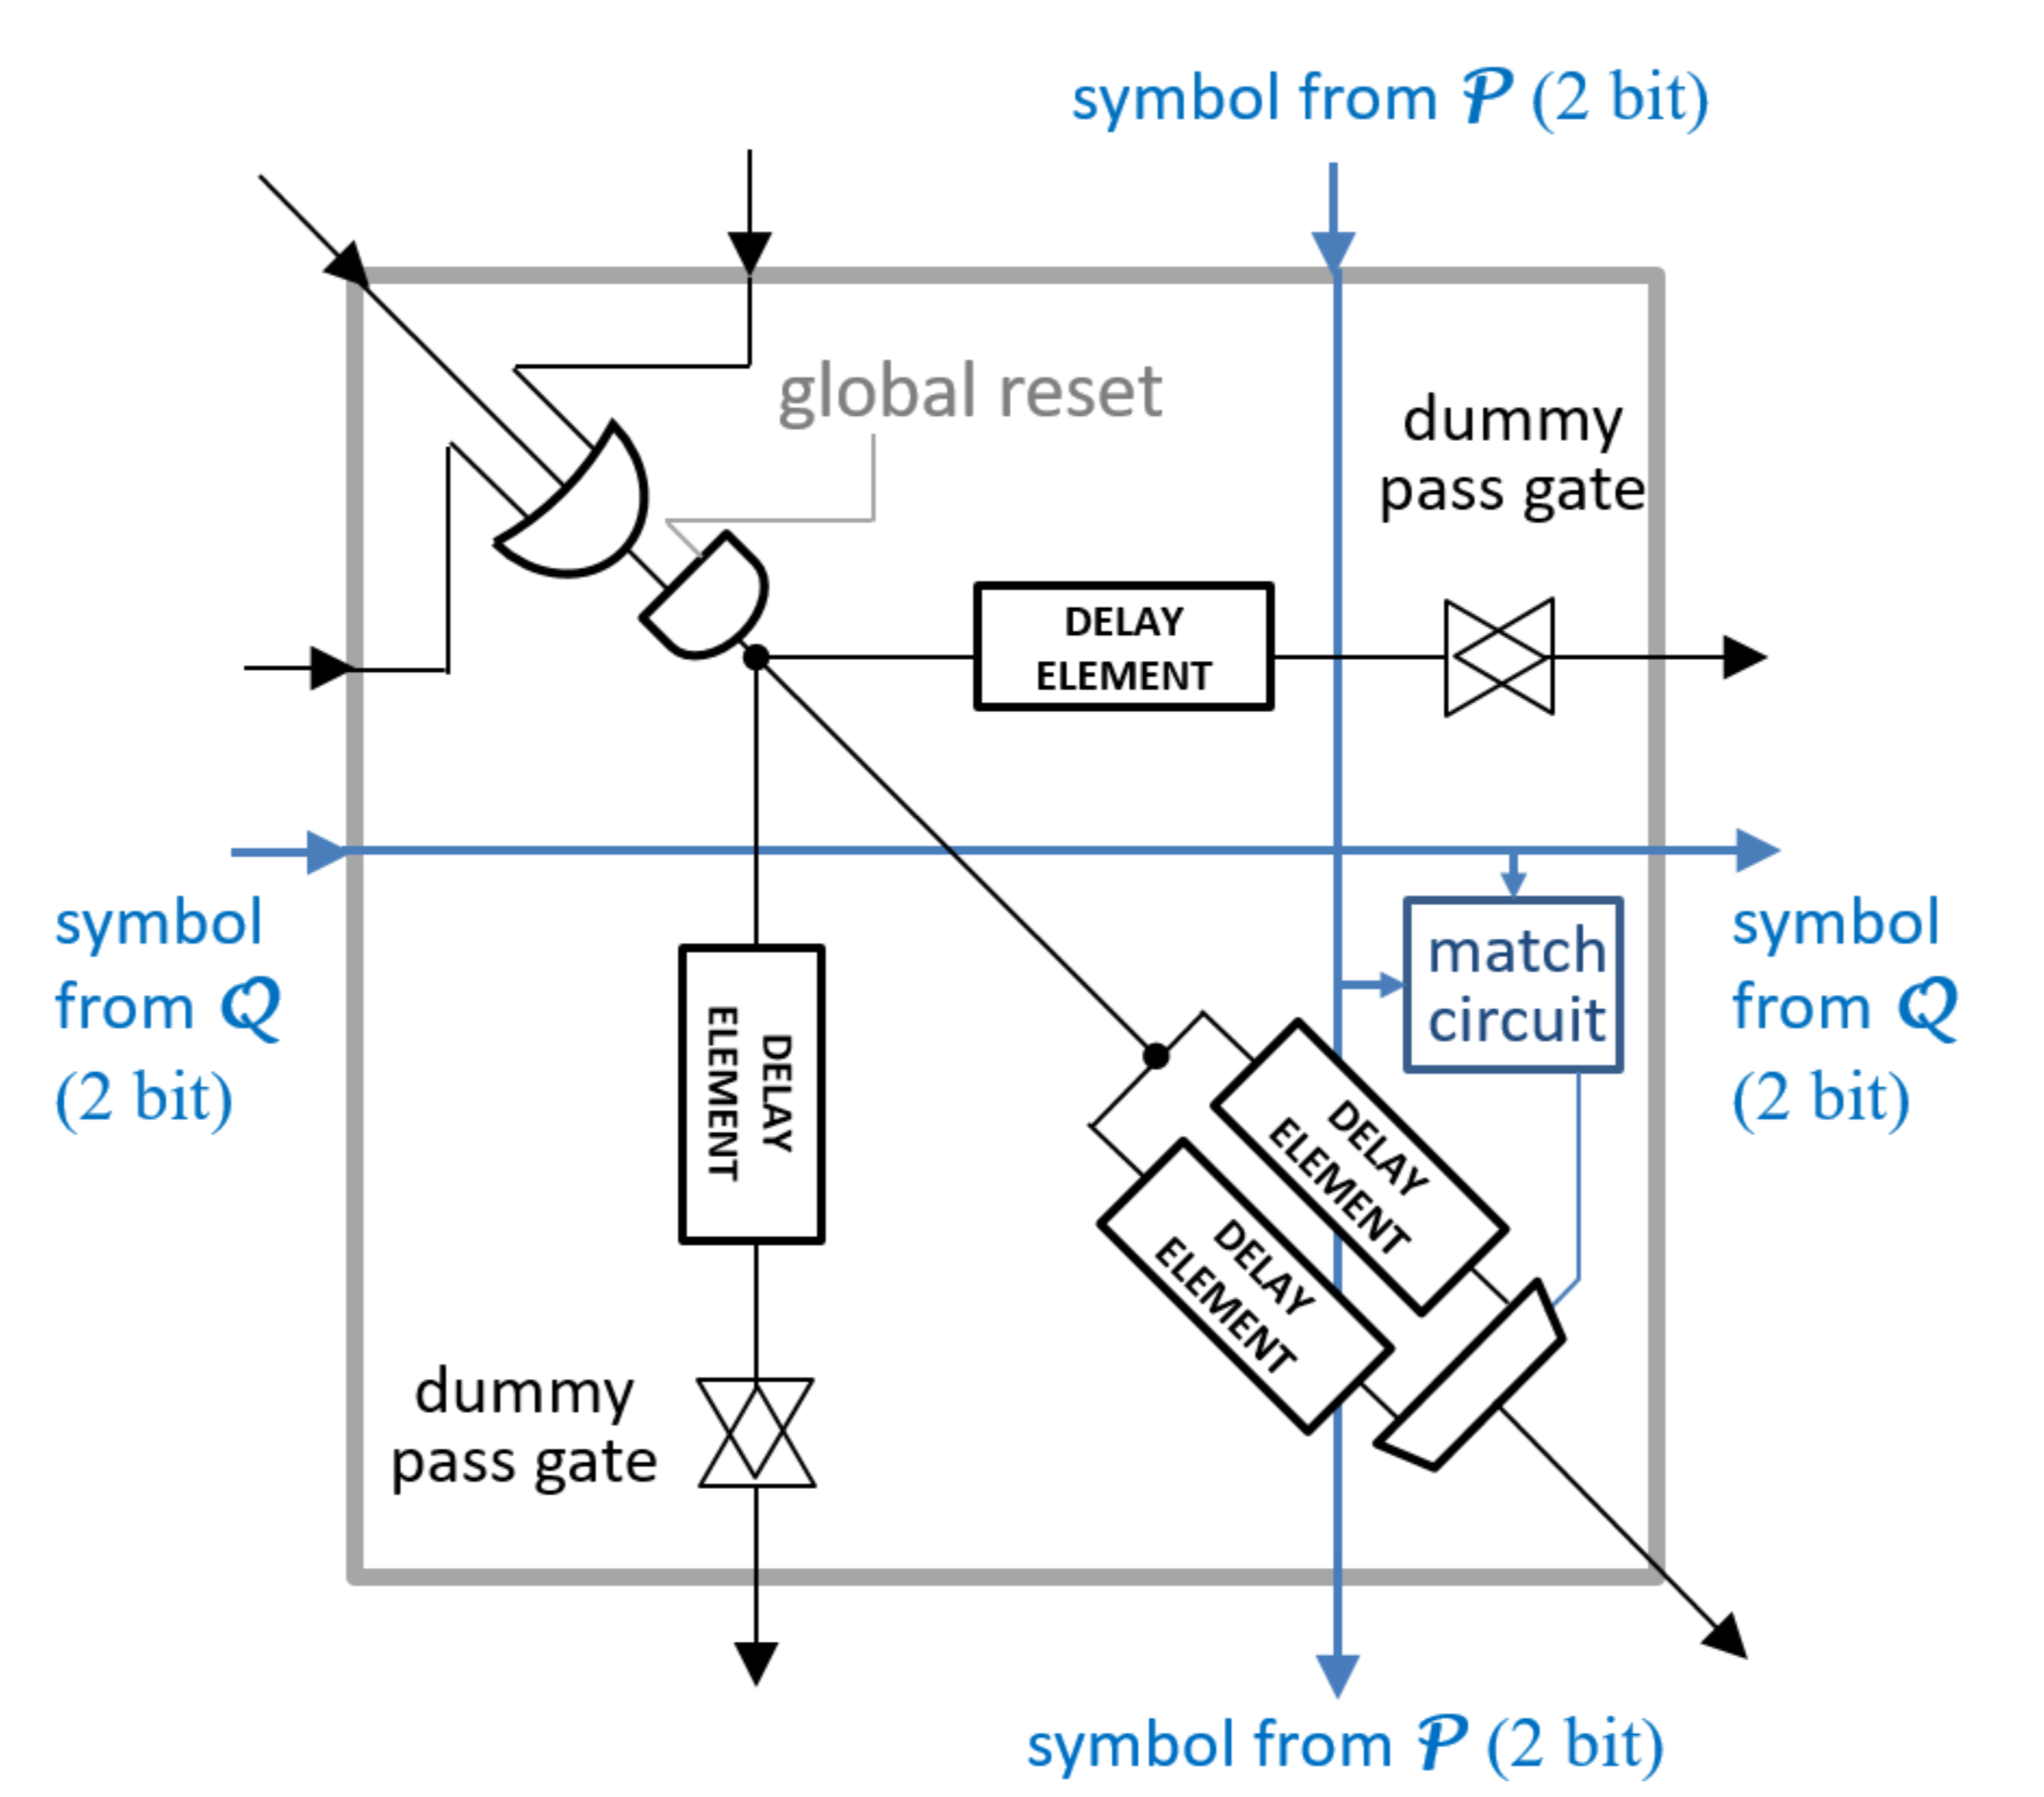
\includegraphics[keepaspectratio,scale=0.3]{fig/2/CMOSasync.png}
\caption{CMOSで実装された非同期型Race Logicのセル構造\cite{madhavan20174}}
\label{fig:CMOSasync}
\end{center}
\end{figure}

ブール値“1”の信号は左・斜上・上のセルのいずれからも入力される.
入力された信号はORゲート,リセットのためのANDゲートを通過する.
アレイのリセットのタイミングは,全ての遅延素子が確実にリセットされるように外部から調整される.
ANDゲートを通過後に次のセルへの伝搬に向けて分けられ,それぞれの経路で遅延素子を通過する.
各着色した経路では遅延素子によって起こる遅延に変化をつけている.
同期型と同様,アルファベットの符号化を入力とするMUXから所望の遅延を選択することができる.
ダミーのパスゲートは,全ての遅延経路に亘って同様の遅延を保証するために斜下へのパス以外に追加されている.

図\ref{fig:CMOSasync}のセルを繰り返した構造を持つアレイに信号が入力された時から出力信号を得るまでの遅延時間をカウントするカウンタがアレイ外部に存在する.
\end{itemize}
上記の回路については,シミュレーションをもってその有効性が明らかにされている.


